\documentclass{article}
\title{Monte Carlo simulation}
\author{Christian, Jonathan, Marcus, Puk \& Sofia }
\date{\today}

\usepackage{listings}
\usepackage{xcolor}
\usepackage{graphicx}
\usepackage{epstopdf}



\definecolor{codegreen}{rgb}{0,0.6,0}
\definecolor{codegray}{rgb}{0.5,0.5,0.5}
\definecolor{codepurple}{rgb}{0.58,0,0.82}
\definecolor{backcolour}{rgb}{0.95,0.95,0.92}

\lstdefinestyle{mystyle}{
	backgroundcolor=\color{backcolour},   
	commentstyle=\color{codegreen},
	keywordstyle=\color{magenta},
	numberstyle=\tiny\color{codegray},
	stringstyle=\color{codepurple},
	basicstyle=\ttfamily\footnotesize,
	breakatwhitespace=false,         
	breaklines=true,                 
	captionpos=b,                    
	keepspaces=true,                 
	numbers=left,                    
	numbersep=5pt,                  
	showspaces=false,                
	showstringspaces=false,
	showtabs=false,                  
	tabsize=2
}

\begin{document}
	
	
	\setcounter{section}{0}
	\maketitle
	\newpage
	\tableofcontents
	\newpage
	
	\section{Introduction}
	
Regression is a tool in statistics used to understand the relationship between one dependent variable and one or more independent variables. For regression to be both accurate and reliable, a set of assumptions needs to be met. These assumptions are independence of errors, linearity, homoscedasticity, normality of errors, multicollinearity, and correct model specifications. If these assumptions are not met, it can introduce bias and inaccuracies in the regression model.
	\newpage
	
	\section{Statistical theory}
	This section will focus on the theoretical background needed to understand how to create regression models, how to test a models reliability and significance, how to generate data and how Monte Carlo Bootstarpping works.

\noindent Sections 3.1 through 3.5 are based on the book 'Probability and Statistics for Engineers and Scientists' \cite{ProbAndStat}. \newline

\noindent Statistics is a field in mathematics, that gives tools to analyze and understand data. Statistics comes in two branches, these are descriptive statistics and inferential statistics. Descriptive statistics is used to describe the general tendencies in some data, such as finding the mean and variance, but no predictions or conclusion are made beyond the data itself. In contrast, inferential statistic is the branch of statistics that makes predictions and generalizations of a population based on a sample, this includes methods such as hypothesis testing and regressions. 

\noindent To address the challenges, when violations in the assumptions of modeling regressions through classical means occur, a fundamental statistical understanding is needed. This section introduces the foundational concept of statistics that is required to understand regression models.


\subsection{Probability space}

The \textbf{sample space}, \textit{S}, is the set of all possible outcomes.
\newline
If a sample space contains a finite number of possibilities or an unending sequence with as many elements as there are whole numbers, it is called a \textbf{discrete sample space}.
\newline
Example: When rolling a standard six-sided die form the discrete sample space, the possible outcomes are $S={1,2,3,4,5,6}$ 
\newline

If a sample space contains an infinite number of possibilities equal to the number of points on a line segment, it is called a \textbf{continuous sample space}.
\break
Example: Measuring the heights of people in a population. This is a continuous sample space, because height can take any real value within a given range. 
\newline
An \textbf{event} is a subset, $A\subseteq S$, of the sample space. The event is the amount that contains all possible events.
An example of a discrete event could be rolling a die and getting an uneven number, this would be the event $A={1,3,5}$.
\newline 
For the continuous event, it could be that a person is between 160 cm and 170 cm tall.
\newline

The probability of an event \textit{A}, $P(A)$, is the sum of the weights of all sample points in \textit{A}.
The probability of the whole sample space is 1, $P(S)=1$
The probability of any event being between 0 and 1,$0<P(A)<1$
The probability of the empty set being 0, $P(Ø)=0$
\newline
\newline
Probability of mutually exclusive events
\newline
If \textit{A} and \textit{B} are mutually exclusive, $A \cap B=Ø$, then
\newline
$P(A \cup B) = P(A)+P(B)$
\newline
\newline
Where \textit{A} and \textit{B} never occur at the same time, so their union is equal to the two events added together. 
\newline
Probability of union
\newline
$P(A \cup B)=P(A)+P(B)-P(A \cap B)$
\newline
Here, the union of the two events is \textit{A} added to \textit{B}, but minus their common event, since it otherwise would be added twice. 
\newline
Two events \textit{A} and \textit{B} are independent, if 
\newline
$P(A|B)=P(A)$
\newline
The equivalent definition to this is:
\newline
Two events \textit{A} and \textit{B} are independent if and only if 
\newline
$P(A \cap B)=P(A)P(B)$
This says that the probability of both event \textit{A} and \textit{B} happening, is equal to the product of the two events.


\subsection{Random Variables}
Now we will introduce random variables, which are important to understand when analysing assumption violations. In statistics, data and results can vary. To understand and handle this randomness, we use random variables, to help describe this uncertainty. \newline

\noindent A random variable is defined as a function that associates a real number with each element in the sample space. We use capital letters to denote a random variabel, for example $X$, and then the corresponding small letter, in this case $x$, for one of its values. As an example we roll a dice 3 times, which gives us a sample space of the different combinations. Each point in the sample space gets a numerical value assigned between 0 and 3.For example, if the random variabel $X$ assumes the number of 5's rolled, then worst case is zero 5's rolled, and best case is three 5's rolled. These values are random quantities assumed by the random variabel $X$, and they are written like this: $X(5,1,2) = 1$ and $X(3,6,1) = 0$.
\newline

\noindent A random variable $X$ can be discrete, which means that its set of possible outcomes is countable. The dice example is a discrete random variable, because you can count how many times 5 is rolled. The outcomes of some statistical experiments may be neither finite nor countable. For example when something is measured such as temperature or speed where the set of possible values is an entire interval of numbers, it is not discrete. The random variable $X$ then takes values on a continues scale, which therefore is called a continuous random variable.

\subsubsection{Discrete Random Variable}
\label{sec:disc}
A discrete random variable can take each of its values with a certain probability. Frequently, it is convenient to represent all the probabilities of a random variable $X$ by a formula. Let $X$ be a discrete random variable which can take the values $x_{1}, x_{2},...$ Then the distribution of $X$ is given by the probability function:

\begin{equation}
	f(x_{i})=P(X=x_{i}),\quad i=1,2,...
\end{equation}
\newline
For a discrete random variable this function is also called the probability mass function, where following holds for each possible outcome $x$:

\begin{itemize}
	\item $P(X = x) = f(x).$
	\item $f(x) \geq 0,$
	\item $\sum_x f(x) = 1.$
\end{itemize}

\noindent In addition to the probability mass function $f$, the discrete random variable $X$ also has a cumulative distribution function $F(x)$ given by:

\begin{equation}
F(x) = P(X \leq x) = \sum_{x_i \leq x} f(x_i), \quad x \in \textbf{R}.
\end{equation}


\noindent This helps decide the probability that the random variable assumes a value equal to or smaller than $x$. Its sums up the probability density functions values.
\newline

\noindent The mean of a discrete variable $X$, with a distribution function $f(x_{i})$ is given by:

\begin{equation}
\mu = E(X) = \sum_i x_i P(X = x_i) = \sum_i x_i f(x_i).
\end{equation}

\noindent The mean is typically the expected value. It is a weighed average of the possible values of $X$. The values are weighed by its probability in the sample space.
\\

\noindent In addition to the mean, we should also mention the variance. The variance is the mean squared distance between the values of the variable and the mean value. It is given by:

\begin{equation}
\sigma^2 = E\left[(X - \mu)^2\right] = \sum_{i} (x_i - \mu)^2 f(x_i)
\end{equation}

\noindent The variance indicates whether the values of $X$ are far from the mean values or close. A high variance means that the values of $X$ have a high probability of being far from the mean values and vice versa. Along with the variance, the standard deviation is also often used. It is given by the square root of the variance:
\begin{equation}
\sigma=+\sqrt{\sigma^2}.
\end{equation}

\noindent The advantage of the standard deviation over the variance is that it is measured in the same units as $X$.

\subsubsection{Continuous Random Variable}
Contrary to a discrete random variable, a continuous random variable can take values that are not countable. A continuous random variable can take infinetly many possible values within a certain range or interval. For a continuous random variable $X$ the distribution is given by the probability density function $f$, which satisfies:

\begin{itemize}
	\item $f(x)$ is defined for all $x$ in $\textbf{R}$,
	\item $f(x) \geq 0$ for all $x$ in $\textbf{R}$,
	\item $\int_{-\infty}^{\infty} f(x) \, dx = 1.$
\end{itemize}

\noindent Condition 3. ensures that $P(-\infty < X < \infty) = 1$, which means that the probability of the random variable $X$ being between $-\infty$ and $\infty$ is 100\%. Furthermore the probability of $X$ assuming a specific value $a$ is zero, in other words: $P(X=a)=0$. That means that the values of the density function should not be interpreted as a probability of a given outcome. Instead the probability of $X$ is found by integrating over the probability density function. So, the probability that a continuous random variable $X$ lies between the values $a$ and $b$ is: 

\begin{equation}
P(a < X < b) = \int_a^b f(x) \, dx.
\end{equation}


\noindent A continuous random variable $X$ also has a distribution function $F(x)$, that also predicts whether $X$ assumes a value equal to or smaller than $x$. For a continuous random variable it is again given by integrating over the probability density function in the interval from $-\infty$ to $x$:
\begin{equation}
F(x) = P(X \leq x) = \int_{-\infty}^{x} f(y) \ dy.
\end{equation}


\noindent That also means $P(a<X<b)$ can be calculated by $F(b)-F(a)$.
\\

\noindent For a continuous random variabel $X$ the mean, variance and standard deviation the same interpretation applies. Just given by different formulars, which are:
\begin{equation}
	\mu = E(X) = \int_{-\infty}^{\infty} x f(x) \, dx
\end{equation}

\noindent and
\begin{equation}
\sigma^2 = E\left[(X - \mu)^2\right] = \int_{-\infty}^{\infty} (x - \mu)^2 f(x) \, dx,
\end{equation}

\noindent (The standard deviation is still given by til square root of the variance).


\subsection{Estimator and estimates}
If we are interested in certain parameters of a population distribution, we can look at a sample. From this, we can make a point estimate. 
\newline
Examples of this are, 
\newline
$\bar{x}$ is a point estimate of $\mu$
\newline
s is a point estimate of $\sigma$
\newline

\noindent This is often supplemented with a confidence interval.
\newline
This is an interval around the point estimate, where we are confident that the population parameter is located.
\newline

\noindent For $\mu$, we have different ways of estimating it. We can use the sample mean $\bar{X}$, or the average $X_T$ of the sample upper and lower quartiles. 
But in this case, we have to look out for bias. If the distribution of a population is skewed, then $X_T$ is biased. The result of this is, that in the long run, this estimator will systematically over or under estimate the value of $\mu$. This is written as,
\newline
$E(X_T) \neq \mu$.
\newline
It is generally preferred that the estimator is unbiased. In this case, $\bar{X}$ is an unbiased estimate of the population mean $\mu$.
\newline

\noindent The standard error of $\bar{X}$ is $\frac{\sigma}{\sqrt{n}}$. Here, the standard error decreases, when the sample size increases. If an estimator has this property, it is called consistent. If we compare, the estimator $X_T$ is also consistent, but has a greater variance than $\bar{X}$. 
\newline
It is generally preferred that the estimator has the smallest possible variance, and in that case it is called efficient. So $\bar{X}$ is an efficient estimator.
\newline
When estimating a parameter, the symbol $\hat{}$ is used above it. For $\mu$, $\hat{\mu} = \bar{X}$ .
\newline
We can calculate $\bar{X}$ using the following formula,
$$\bar{X}=\frac{1}{n} \sum_{i=1}^{n}X_i$$   
\newline
For the variance $\sigma$, we can estimate it by using the formula for $S^2$,
$$S^2=\frac{1}{n-1} \sum_{i=1}(X_i-\bar{X})$$
\subsection{Probability distribution}
Data can come in various distributions depending on different parameters such
as degrees of freedom. The distribution is the shape of the data and it will have
an effect on statistical models. Therefore it is important to have an understanding of distributions.
\subsubsection{Normal distribution}
In the world of statistics, the most common distribution is the normal distribution. It is constructed as a bell shape. The normal distribution is a continuous distribution, with this density function:
$$n(x;\mu,\sigma) =\frac{1}{\sqrt{2\pi\sigma}}e^{-\frac{(x-\mu)}{2\sigma^2}}$$
The distribution is dependent on the mean($\mu$) and the standard deviation($\sigma$), where changes to the mean will result in a change in the positioning of the normal distribution. Whereas a change in the standard deviation will change the spread of the curve. The normal distribution also always contains an area under the curve that is equal to one. This is to ensure that the normal distribution correctly models probability.

There is a special case of the normal distribution, called the standard normal distribution, where the mean is zero and the standard deviation is one. All variations of a normal distribution can be standardized by a transformation of the distribution, using the Z-score formula.
\newline
$$Z=\frac{X-\mu}{\sigma}$$
\newline
$Z$ in the Z-score represents the amount of standard deviations a given $X$ value, deviates from the mean.

\subsubsection{The central limit theorem}
A very effective theorem in statistics is the central limit theorem. This theorem states that if a random sample $\overline{X}$, with the size $n$, is taken from a population with a mean and a finite variance, then as $n$ goes towards infinity, the distribution will resemble a normal distribution. If used with the Z-score formula, the distribution will resemble a standard normal distribution. The formula for the Z-score, when in conjunction with the central limit theorem, looks like this:
$$Z=\frac{\overline{X}-\mu}{\sigma/\sqrt{n}}$$
Where $\overline{X}$ is a random sample of size $n$ and $\mu$ is the mean of the true population. The standard error i represented by $\sigma/\sqrt{n}$, where $\sigma$ is the standard deviation and $n$ is the sample size.
Usually the standard deviation is unknown, for these situations it's possible to use the estimator $S^2$. This estimates the variance of the population from the variance of the sample, by this formula:
$$s^2=\sum_{i=1}^{n}\frac{(x_{i}-\overline{x})}{n-1}$$

The square root of the variance is the standard deviation, therefore the square root of the estimator $S^2$ would be the estimated standard deviation. The problem with using the estimator $S^2$, is that with small samples the variance is small and therefore it contains a lot of bias. In this situation the t-distribution would be used instead of the normal distribution, because the t-distribution takes the bias into account the bias of the standard deviation. It does this by having thicker tails, meaning that the probability of more extreme values are higher.

\subsubsection{The t-distribution}
The t-distribution is shaped as the standard normal distribution, in a bell shape and symmetrical around the mean of zero, the difference is that the t-distribution is more variable. This comes from the fact that the t-distribution is dependent on the degrees of freedom. When the degrees of freedom surpasses 30, the rule of thumb is that the distribution will resemble a normal distribution. So before 30 degrees of freedom, the distribution contains more variance.
The t-distribution will come to resemble the standard normal distribution, when in surpasses 30 degrees of freedom, this makes sense, since the two distributions have the same formula:
$$T=\frac{\overline{X}-\mu}{S/\sqrt{n}}$$

The only difference is the estimated standard deviation $S$.
\newpage
\subsection{Statistical methods}

\subsubsection{Confidence intervals}
The confidence interval is a good tool to use, when trying to estimate a parameter of a population. Its used to create an interval, where the parameter has a probability to lie inside of. This probability is called the confidence level and it's a chosen value, usually the chosen confidence level is either 95\% or 99\%. The confidence interval will become bigger with a larger confidence level. A good confidence interval is small with a large confidence level, this will usually occur when the sample size is large. The chosen confidence level relates to an $\alpha$-value, where as an example the chosen confidence level is 95\%, then the $\alpha$-value would be 5\% or normally written as $0.05$. The $\alpha$-value will sometimes be needed to find the critical value, that is used to calculate the margin of error, as an example it's used when trying to find the critical value of the confidence interval, when working with a t-distribution.
\newline
To set up a confidence interval, the margin of error needs to be computed and then that will be both added and subtracted from the point estimate. This will give the values of the outer bounds of the interval. The margin of error is calculated from this formula:
$$Margin\_of\_error = critical\_value \pm standard\_error$$
\newline
The standard error will change depending on which parameter that the confidence interval is estimating, but the general formula for the standard error is:
$$\frac{\sigma}{\sqrt{n}}$$
\newline
An example of computing a confidence interval of the mean while working with a standard normal distribution, then the formula for the confidence interval would be this:

$$P(-z_{\alpha/2}<Z<z_{\alpha/2}) = 1-\alpha$$
\newline
Where $1-\alpha$ is the confidence level. As it's the mean that is being estimated, then instead of Z-score, then $\mu$ must be isolated and that is done by multiplying $\frac{\sigma}{\sqrt{n}}$ and subtracting $\bar{X}$ on all sides, then multiplying all side by $-1$ to remove the minus sign. So the formula for a confidence interval of the mean will look like this:

$$P(\bar{X}-z_{\alpha/2}\frac{\sigma}{\sqrt{n}}<\mu<\bar{X}+z_{\alpha/2}\frac{\sigma}{\sqrt{n}})=1-\alpha$$
\newline
This formula will give the upper and lower bounds of the confidence interval.\\

\noindent \textbf{The interpretation of a confidence interval}
\newline
To interpret a confidence interval, it would be incorrect to interpret the confidence level of some value $x$, as the probability of the true parameter being inside of the interval. The reason behind this is that the computed interval is static, so either the value $x$ is inside the interval or it's not. So the correct way of interpreting the confidence interval is by taking multiple samples and computing the confidence interval for all samples, then the value $x$ would reside inside 95\% of the confidence intervals.
\textbf{Kilde for fortolkningen af kofidense intervaller:}
\newline
$http://www.drhuang.com/science/mathematics/book/probability_and_statistics_for_engineering_and_the_sciences.pdf$


\subsubsection{Hypothesis testing}
A hypothesis test is used to test an assumption about a population. This is done from a sample of the population, as the information about the population is usually hard to come by. A hypothesis test is set up, by having a null hypothesis and an alternate hypothesis.
$$H_0 = Null\; hypothesis$$
$$H_a = Alternate\; hypothesis$$
When working with hypothesis testing, the hypothesis $H_0$ is usually represented as the status quo, where as the hypothesis $H_a$ is represented as the opposition. It is also important to note that there is only two outcomes of a hypothesis test, either $H_0$ is rejected in favor of $H_a$ or $H_0$ is failed to be rejected. Therefore in no situation can $H_0$ be stated to be an absolute truth, as there might be other samples where $H_0$ will be rejected. Therefore in a hypothesis test $H_0$ needs to be the thing that can be rejected and if $H_0$ gets rejected, then $H_a$ will become the new status quo until proven otherwise.\\
In a hypothesis test $H_0$ will be the assumption that a parameter for two populations is the same, where as $H_a$ can be either one of three assumptions, depending on the intention of the hypothesis test.
$$H_0: \theta = \theta_0$$
$$1.\;H_a: \theta \neq \theta_0$$
$$2.\;H_a: \theta < \theta_0$$
$$3.\;H_a: \theta > \theta_0$$
When the direction of the rejection is not important and also is unknown, then (1) will be the case. This scenario sets up a two-tailed-test, where the hypothesis test is used to reject $H_0$ if $H_a$ is either significantly larger or smaller than $H_0$, this means that the critical area is on both sides of the difference of $\theta$ and $\theta_0$. Either (2) or (3) will set up a one-tailed-test, where depending on what is important, either the hypothesis test is used to determine if $H_a$ is significantly bigger or smaller than $H_0$. This means that the critical area only spans one side of the difference between $\theta$ and $\theta_0$.\\

\newline
\noindent \textbf{Error in hypothesis testing}
\newline
When making a hypothesis test there is four different possible outcomes. The results are separated by correct decisions and errors. There exist two types of hypothesis errors, called type 1 error and type 2 error. The type 1 error occurs when $H_0$ is mistakenly rejected and $H_0$ is true. Type 2 error is the opposite, where $H_a$ is rejected and $H_a$ is true. The types of outcomes occurring from a hypothesis test can be seen in Table \ref{tab:example2x3}
\begin{table}[h!]
	\centering
	\begin{tabular}{|c|c|c|}
		\hline
		 & $H_0$ is true & $H_0$ is false \\
		\hline
		Does not reject $H_0$ & Correct decision & Type 2 error \\ \hline
		Reject $H_0$ & Type 1 error & Correct decision \\
		\hline
	\end{tabular}
	\caption{Outcomes of a hypothesis test}
	\label{tab:example2x3}
\end{table}

It is possible to compute the possibility of a type 1 error occurring, because the probability is equal to the significance level also denoted as $\alpha$. So when a significance level of 0.05 is chosen, then that is the same as the probability of a type 1 error occurring. As for computing the probability of a type 2 error occurring, it can only be done if $H_a$ is defined. The probability of a type 2 error occurring is denoted as $\beta$ and by a defined $H_a$, whats meant is that the $\mu$ of the sample is needed. Depending on the distribution and sample size, the calculation of $\beta$ will change.
As an example in a normal distributed sample, the $\mu$ is needed in calculating a Z-score and this Z-score is needed to extract a value from the Z-table. Then the probability of a type 2 error occurring is calculated from this formula:
$$
\beta = 1-\phi(Z_\beta)
$$
In this formula $\phi(Z_\beta)$ is the value from the Z-table. Its possible to reverse this formula and denote the probability of a correct decision, where $H_0$ is rejected and $H_a$ is true, this is denoted as, $1-\beta$.
It is possible to change the probability of these two errors occurring, this is done by changing the significance level. The consequence of this is that one of the errors will always lower its probability of occurring, while the other will have its probability increased. By reducing the significance level, the type 1 error will have a lower probability of happening, but a type 2 error will have an increase in probability of occurring. The opposite where the significance level is increased, the probability of the type 1 error will increase and for the type 2 error, it will be reduced. To overcome this problem, the only solution is to increase the sample size, as this will lower the probability of either of the two error types of happening.





	\newpage
	
	\section{Polynomial regression}
 	\input(Polinomial regression)
	\newpage
	
	\subsection{Assumptions}
	\newpage
	
	\section{Pseudo random number generator}
	When producing a synthetic dataset, there is a need for a lot of random numbers. Many programming languages have a built-in function that produces numbers that appear random, but actually are not. Computers are deterministic machines, and therefore cannot produce a number without some sort of algorithm. If the algorithm is known, it becomes possible to predict the next number; hence the numbers are not completely random. Random numbers should be independent; that is, each number should have no connection to any previously produced values. The distribution should also be uniform, meaning if you generate 1,000,000 random numbers in the range [0,1), you'd expect about 500,000 values in [0, 0.5) and about 500,000 in [0.5, 1). Earlier in history, these numbers have been produced by flipping coins or rolling dice. Today, it is possible to produce truly random numbers by using atmospheric noise. Despite its potential advantages, this method requires significant resources, making it inefficient for the intended application. Therefore, pseudo-random numbers will be used instead.
\newline

\noindent Pseudo-random numbers behave like random numbers but are deterministically generated from a seed value. While
these numbers are not truly random, they are sufficiently unpredictable for many practical applications.
To generate the data, we use a Pseudo-Random Number Generator (PRNG).
PRNGs are algorithms that produce sequences of numbers that appear random.
\newline

\noindent Random numbers are widely used in fields such as statistics, game theory, cryptography, and simulations. These applications require numbers that behave
as if they were random, yet can be reproduced when needed. This is where
PRNGs come in. They allow for repeatable randomness, making them ideal for
controlled experiments, testing, and security.
\\
This chapter will explore the key concepts behind PRNGs. Before going into the
mechanics of these generators, it is important to first understand what ’random’
means and the characteristics that define truly random numbers.

\subsection{Properties of PRNGs}

The quality of a PRNG is determined by several key factors that influence its
use for different applications. Some of the properties of a good PRNG are independence, a long period and reproducibility
\newline \\
The numbers produced by the PRNG should be statistically independent, en-
suring that each generated value exhibits no correlation with previous numbers
or other sequences. This implies that knowledge of previously generated num-
bers or sequences provides no advantage in predicting the next output.
\newline \\
A PRNG operates within a specific interval before its sequence begins to repeat.
A high-quality PRNG has a long interval, delaying repetition and enhancing its
unpredictability. Conversely, a PRNG with a shorter period becomes more pre-
dictable and less suitable for practical use.
\newline \\
A key feature of a PRNG is its ability to reproduce the same sequence of num-
bers when given a specific seed. This property is particularly useful in testing
and simulation scenarios, where it is essential to generate identical sequences
multiple times for consistency and reproducibility.
\newline \\
In addition, a PRNG must be fast and efficient to prevent it from introducing
performance bottlenecks within an application. The speed of number generation
directly impacts computational efficiency, especially in applications requiring a
large volume of random numbers. An inefficient PRNG can significantly slow
down processes, undermining the overall performance of the system. Therefore,
balancing randomness and efficiency is essential for practical applications

\subsection{Linear Congruential Generator}

Linear Congruential Generator (LCG) is a commonly used approach to generate
pseudo-random numbers. LCG generates a sequence of numbers using a linear
recurrence relation, expressed as:

$$X_{n+1} = (aX_n + c) \bmod m.$$  \\
\\
\noindent $X_0$ is the seed value and must be in the range $0 \leq X_0 < m$ \newline
$a$ is the multiplier,\newline 
$c$ is the increment and \newline
$m$ is the modulus, which specifies the range of values. $m$ must be greater than 0 \newline
\\
\noindent The operation 'mod $m$' represents division by $m$, where only the remainder
is retained. This ensures that the generated number remains within the range
0 to $m-1$.  $X_0$, $a$ and $c$ must all be in the interval $[0, m)$. 
Here is an example of the first 4 numbers of a sequence given these parameters: \newline

\begin{center}
	$a = 5$, $c = 1$, $m = 16$, and $X_0 = 7$:
\end{center}

$$X_1 = (5 \cdot 7 + 1)\bmod 16 = 4 $$
$$X_2 = (5 \cdot 4 + 1) \bmod 16 = 5 $$
$$X_3 = (5 \cdot 5 + 1) \bmod 16 = 10 $$
$$X_4 = (5 \cdot 10 + 1) \bmod 16 = 3 $$
\\
\noindent This sequence has a period of 16. In an LCG, the period can be as large as $m$,
because the remainder after division by $m$ will always be less than or equal to
$m$. Consequently, choosing a large $m$ is typically desirable, as it can potentially
lead to longer periods. However, the period length is not determined solely by
$m$; the choice of other parameters—such as the multiplier, increment, and the
seed, along with their relationships, significantly impact the overall period. It
is possible to select a larger $m$ and still end up with a shorter period if the parameters are not chosen properly. Here is an example where a larger $m$ results in a shorter period, illustrating that.

\begin{center}
	$a=4$, $c=6$, $m=20$, $X_0=3$
\end{center}

$$X_1=(4 \cdot 3 +6)=18 \bmod 20=18$$ 
$$X_2=(4 \cdot 18+6)=78 \bmod 20=78 \bmod 20=18$$

\noindent Here a larger $m$ is used, but a shorter period of 1 appears. 
\newline \\
The selection of the optimal parameters for a LCG would be excessive for the objective of this project, it is beyond the scope of this project and will therefore not be addressed further.

\subsection{Test of PRNG}
As stated previously, the length of the sequence produced by the PRNG is not the only important factor. A uniform distribution and independence of each generated number is significant too. If these criteria are not met, there will be correlation between the generated numbers, which means that the randomness is of low quality. For example, consider a sequence that follows the three-times-table, with the first number being 3: (3,6,9,12,...). In that sequence, it is pretty easy to guess the upcoming number, based on the previous one. Normally the correlations are harder to spot than this example, which is why it is important to test the quality of a PRNG.
\newline

\noindent There are different tests used to evaluate PRNG quality and performance, including the Kolmogorov-Smirnov test, chi-squared test and the spectral test. Passing one of these tests does not mean that it will pass others. Therefore, every test that it passes, just makes it more likely to produce a high quality sequence. One of the important tests for LCG is the spectral test. Another advantage of the spectral test in the context of this paper is that it can be visualized in two or three dimensions, which can make it easier to understand.
\newline

\noindent The test looks at how the numbers in the sequence are distributed in different dimensions. If hyperplanes and lines occur, as seen on Figure \ref{fig:badspec2d} and Figure \ref{fig:badspec3d}, generated by $X_{n+1}=137\cdot X_{n}+187$ mod $256$, the sequence fails the test, since the distribution is not random.
\newline

\noindent Looking at the spectral test used on a LCG with better parameters:  $X_{n+1}=3 141 592 621\cdot X_{n}+1$ mod $2^{32}$ (Kilde: Knuth), on Figure \ref{fig:goodspec2d} and Figure \ref{fig:goodspec3d}, the hyperplanes will not always be visible in 2d or 3d, but only in higher dimensions. Therefore a visual examination will not be enough to conclude the complete quality of a PRNG. Methods for inspecting LCGs in these dimensions do exist, but will not be mentioned in this project
\newline

\noindent In this project, the PRNG used will be the Mersenne-Twister. It has very good properties, uniformity and a period of $2^19937-1$ and passes the spectral test. The test in 2D and 3D can be seen on figure \ref{fig:msspec2d} and figure \ref{fig:msspec3d}. Another reason for this choice is that Mersenne-Twister is the built-in generator in R, which makes it convenient. 
\newpage

%Spectral test for bad LCG
\begin{figure}
	\centering
	\begin{minipage}{0.45\textwidth}
		\centering
		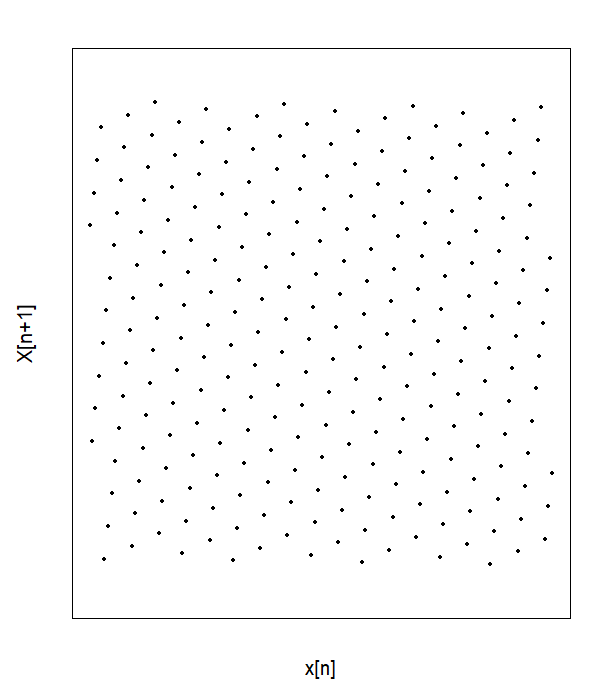
\includegraphics[width=\linewidth]{billder/spec_bad_lcg_2d.png}
		\caption{2D spectral test for LCG using bad parameters: $X_{n+1}=137\cdot X_{n}+187$ mod $256$}
		\label{fig:badspec2d}
	\end{minipage}\hfill
	\begin{minipage}{0.45\textwidth}
		\centering
		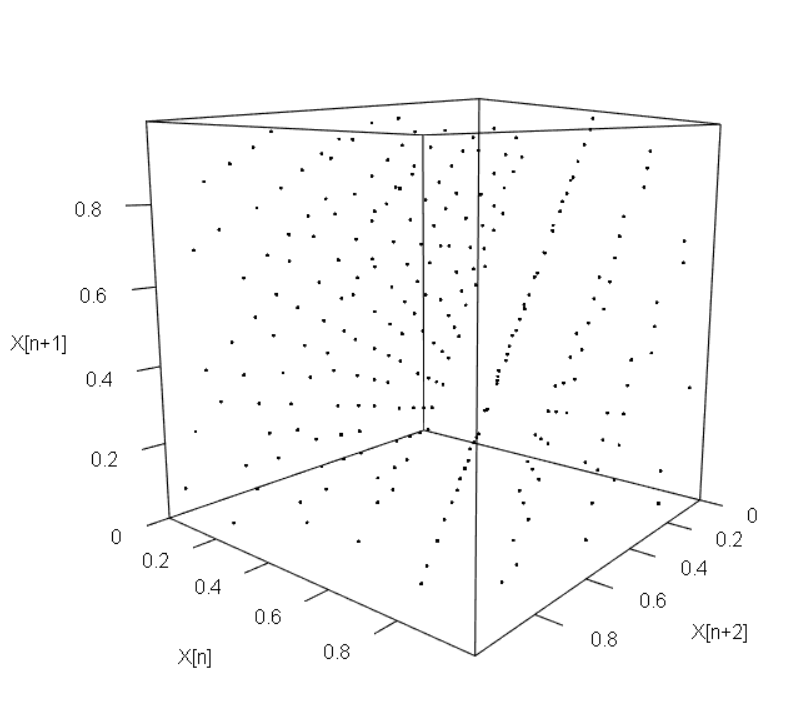
\includegraphics[width=\linewidth]{billder/spec_bad_lcg_3d.png}
		\caption{3D spectral test for LCG using bad parameters: $X_{n+1}=137\cdot X_{n}+187$ mod $256$}
		\label{fig:badspec3d}
	\end{minipage}
\end{figure}

%Spectral test good LCG
\begin{figure}
	\centering
	\begin{minipage}{0.45\textwidth}
		\centering
		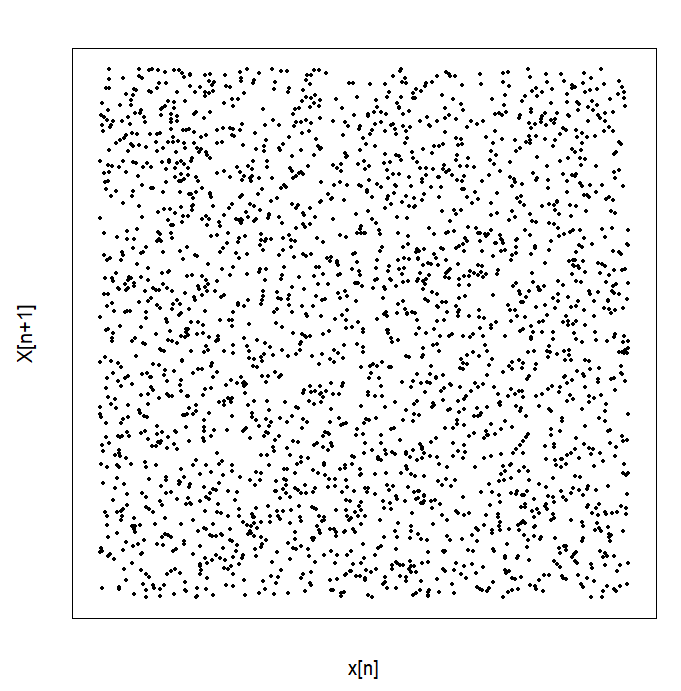
\includegraphics[width=\linewidth]{billder/spec_good_lcg_2d.png}
		\caption{2D spectral test for LCG using good parameters: $X_{n+1}=3 141 592 621\cdot X_{n}+1$ mod $2^{32}$}
		\label{fig:goodspec2d}
	\end{minipage}\hfill
	\begin{minipage}{0.45\textwidth}
		\centering
		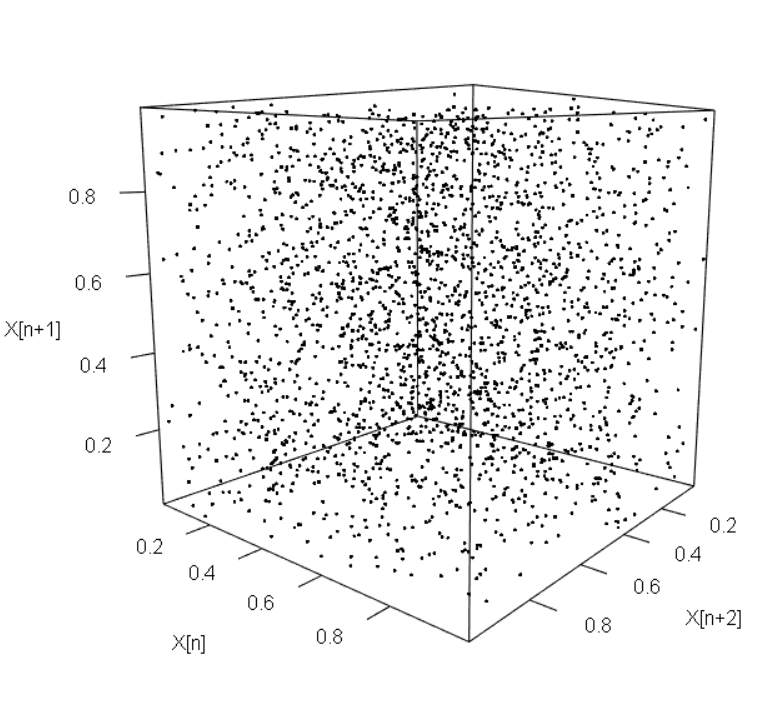
\includegraphics[width=\linewidth]{billder/spec_good_lcg_3d.png}
		\caption{3D spectral test for LCG using good parameters: $X_{n+1}=3 141 592 621\cdot X_{n}+1$ mod $2^{32}$}
		\label{fig:goodspec3d}
	\end{minipage}
\end{figure}

%Mersenne-Twister spectral tests
\begin{figure}
	\centering
	\begin{minipage}{0.45\textwidth}
		\centering
		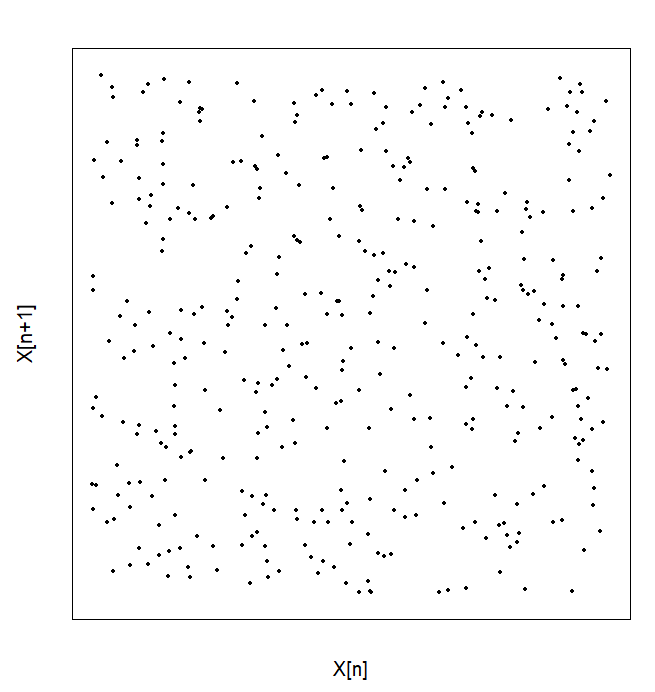
\includegraphics[width=\linewidth]{billder/ms_spec_2d.png}
		\caption{2D Spectral test for the PRNG Mersenne-Twister, in R}
		\label{fig:msspec2d}
	\end{minipage}\hfill
	\begin{minipage}{0.45\textwidth}
		\centering
		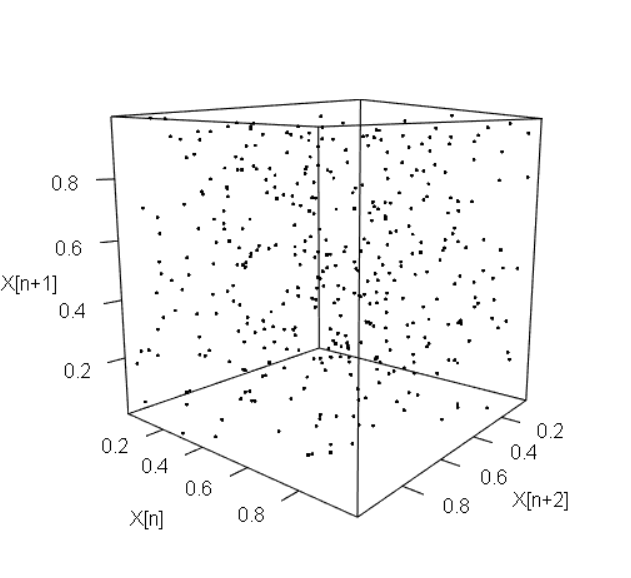
\includegraphics[width=\linewidth]{billder/ms_spec_3d.png}
		\caption{3D Spectral test for the PRNG Mersenne-Twister, in R}
		\label{fig:msspec3d}
	\end{minipage}
\end{figure}

	\newpage
	
	\section{Monte Carlo}
	\subsection{Assumptions}
	\newpage
	
	\section{Problem statement}
	\newpage
	\section{intro til data}
	
\definecolor{codegreen}{rgb}{0,0.6,0}
\definecolor{codegray}{rgb}{0.5,0.5,0.5}
\definecolor{codepurple}{rgb}{0.58,0,0.82}
\definecolor{backcolour}{rgb}{0.95,0.95,0.92}

\lstdefinestyle{mystyle}{
	backgroundcolor=\color{backcolour},   
	commentstyle=\color{codegreen},
	keywordstyle=\color{magenta},
	numberstyle=\tiny\color{codegray},
	stringstyle=\color{codepurple},
	basicstyle=\ttfamily\footnotesize,
	breakatwhitespace=false,         
	breaklines=true,                 
	captionpos=b,                    
	keepspaces=true,                 
	numbers=left,                    
	numbersep=5pt,                  
	showspaces=false,                
	showstringspaces=false,
	showtabs=false,                  
	tabsize=2
}

\lstset{style=mystyle}
	
	To determine whether the data set meets the assumption of homoscedasticity, a scatter plot between the dependent and independent variables is created. It becomes apparent that the variables displacement, weight, and acceleration are not homoscedastic.Furthermore, MPG, displacement, weight, and acceleration are continuous numeric variables, while cylinders, model year, and origin are discrete numeric variables. Additionally, a heat map of the correlation between variables is created to determine if multicollinearity is present among the independent variables. Here, it is apparent that weight, displacement, and cylinders are highly correlated, and that all three are highly correlated with MPG. It is also clear from observing the density functions of the independent variables that none of them, except acceleration, are normally distributed. 
%	\lstinputlisting[language=R, caption=intro til data]{kode/intro.R}



\begin{figure}[h] 
	\centering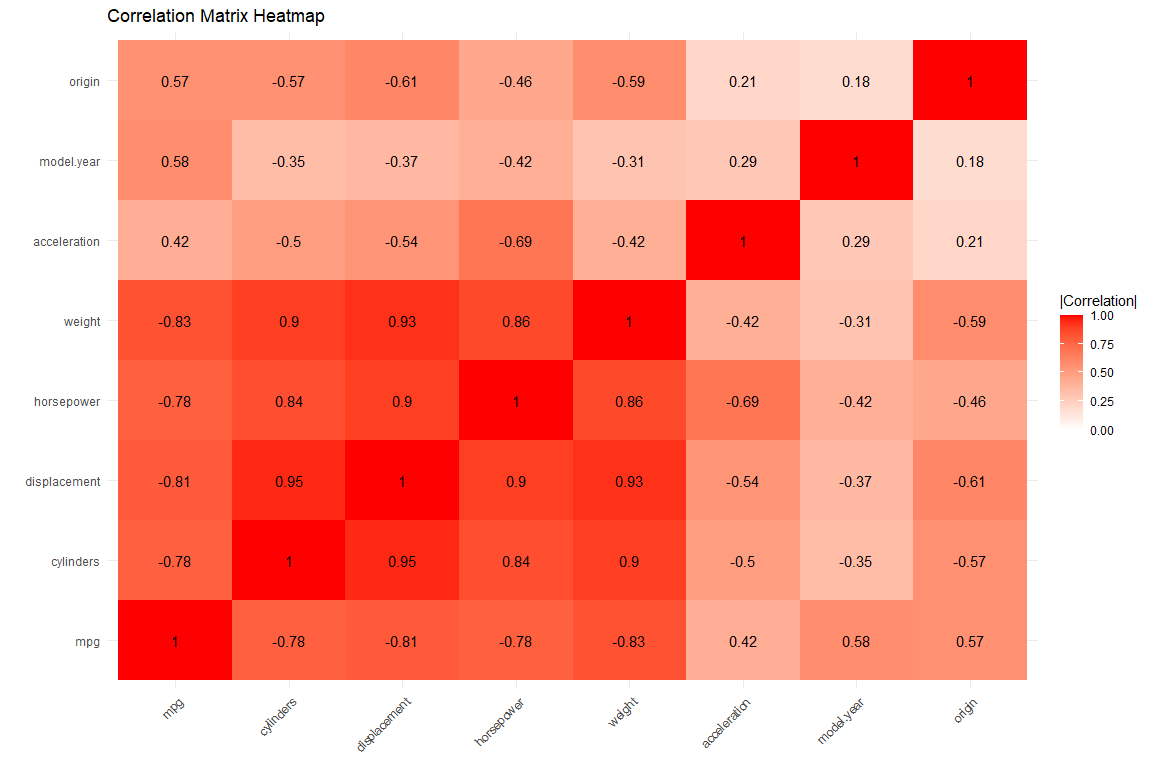
\includegraphics[width=14cm]{billder/1.png}
	\caption{heatmap}
	\label{fig:intro1}
\end{figure}


\begin{figure}[h] 
	\centering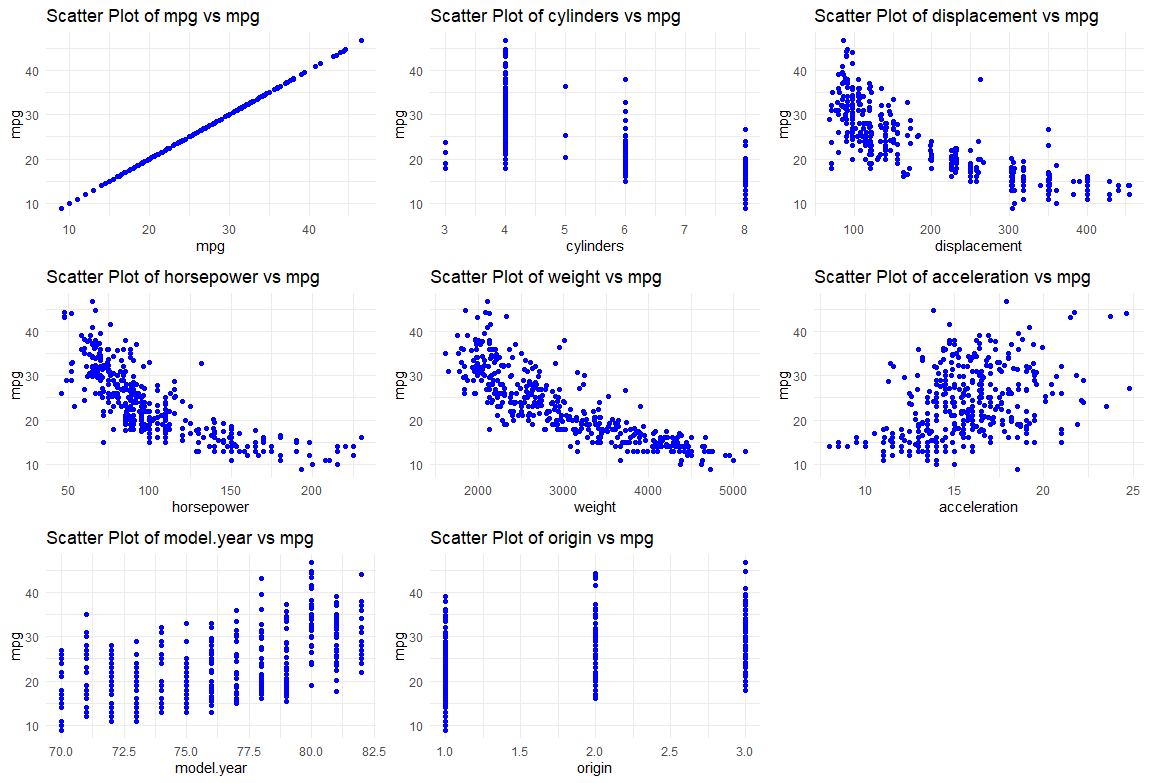
\includegraphics[width=14cm]{billder/2.png}
	\caption{scatterplot}
	\label{fig:instro2}
\end{figure}

\begin{figure}[h] 
	\centering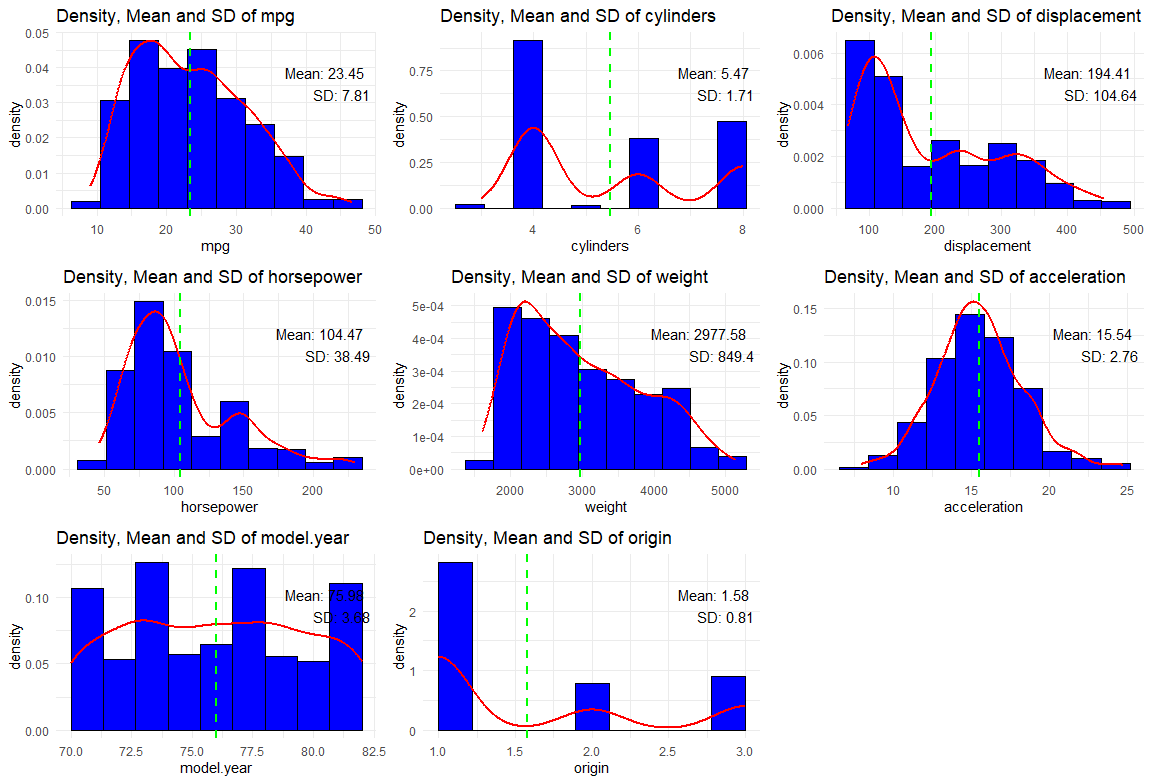
\includegraphics[width=14cm]{billder/3.png}
	\caption{density,mean and sd}
	\label{fig:intro3}
\end{figure}


	\newpage
	\section{Classical regression}
	\newpage
	
	\section{Monte Carlo regression}
	\newpage
	
	

\section{montecarlo bootstrapping }

Monte Carlo bootstrapping is used to find the model for the mpg data. It starts by cleaning the data, then selecting the numeric columns, and defining the Monte Carlo bootstrapping function. After that, it defines the polynomial regression function using mpg as the dependent variable. Next, it defines the simulation function using clusters, thereby speeding up the computation time with the doParallel library. After defining the run simulation function, it runs the simulation with the set seed, simulation number, and sample size of the Monte Carlo bootstrapping method.

After that, it creates histograms of the simulation results. It calculates the mean result of the coefficients, and using these means, it calculates a new regression model and the R-squared of the new average model. Finally, it makes a scatter plot showing the final regression model results versus the results from the actual data set.
%\lstinputlisting[language=R, caption=montecarlo bootstrapping]{kode/montecarlo bootstrapping.R}

\begin{figure}[h] 
	\centering
	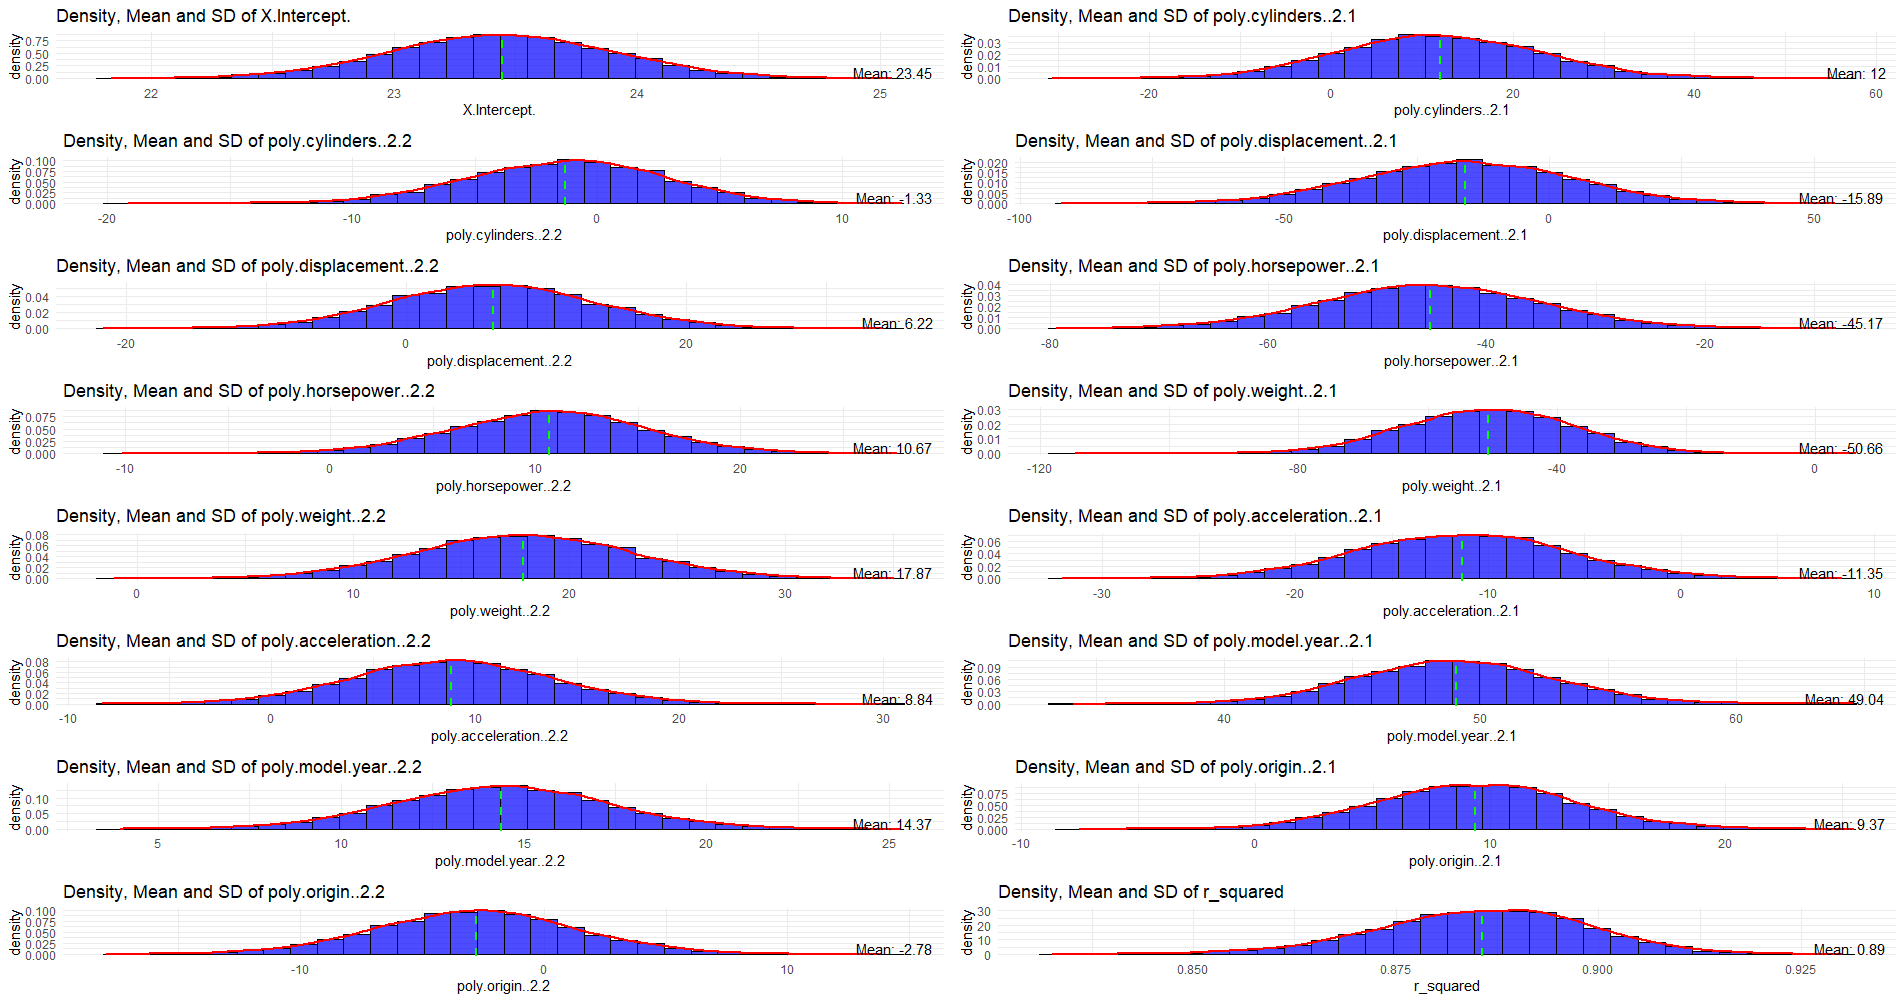
\includegraphics[width=14cm]{billder/10.png}
	\caption{AQI gennem årene.}
	\label{fig:j06}
\end{figure}

%\begin{figure}[h] 
%	\centering
%%	\caption{AQI gennem årene.}
%	\label{fig:j06}
%\end{figure}
	
	
		\section{super syntetisk}
	\section{super syntetisk }

To show the consequences of violating the assumption of homoscedasticity, a dataset is generated with and without homoscedasticity. It starts with generating four normally distributed independent variables using a random number generator. Then, the dependent variable is generated as a function of the four independent variables. A regression model is fitted, and the model is tested. After this, homoscedasticity is violated by adding an error term that scales with the dependent variable. The model is tested again, and it becomes apparent what the consequences of violating the assumption of homoscedasticity are.

\lstinputlisting[language=R, caption=super syntetisk data]{C:/Users/Jonathan/Documents/GitHub/P2/R kode/super syntetisk data_.R}



\begin{figure}[h] 
	\centering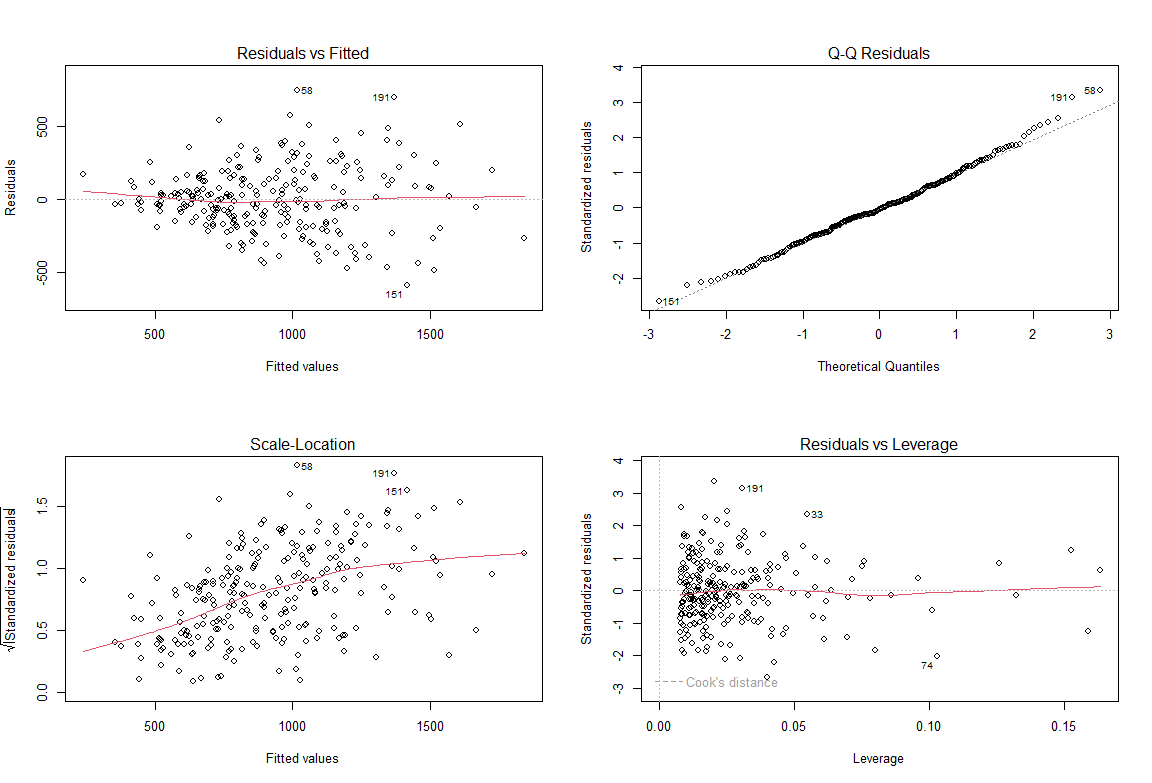
\includegraphics[width=14cm]{p2/4.png}
	\caption{residualplot}
	\label{fig:j06}
\end{figure}

\begin{figure}[h] 
	\centering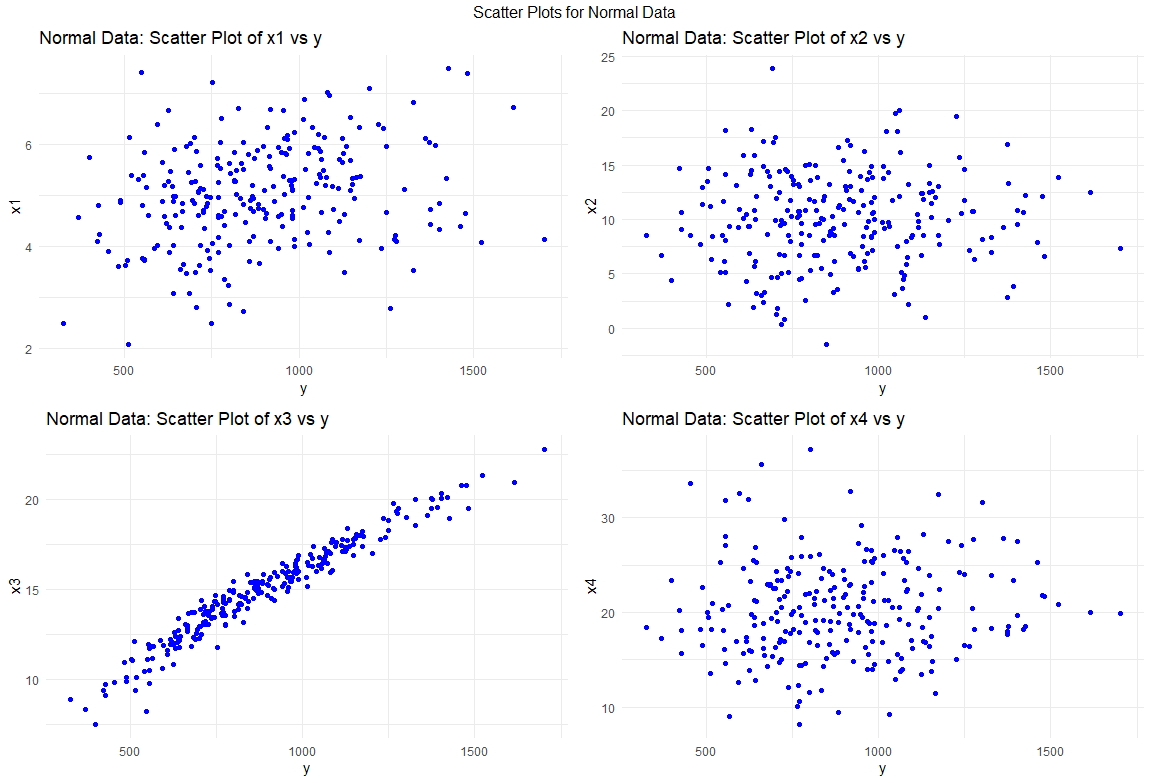
\includegraphics[width=14cm]{p2/5.png}
	\caption{scatterplot.homo}
	\label{fig:j06}
\end{figure}

\begin{figure}[h] 
	\centering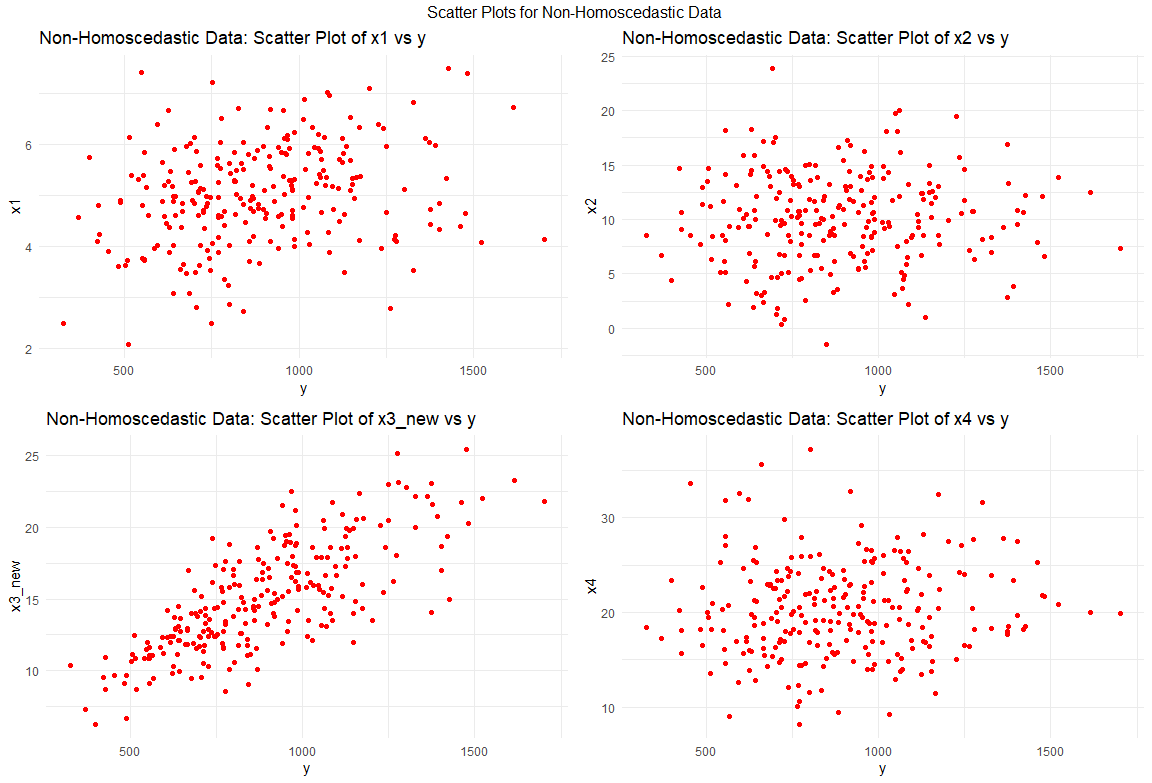
\includegraphics[width=14cm]{p2/6.png}
	\caption{scatterplot.hetro}
	\label{fig:j06}
\end{figure}

\begin{figure}[h] 
	\centering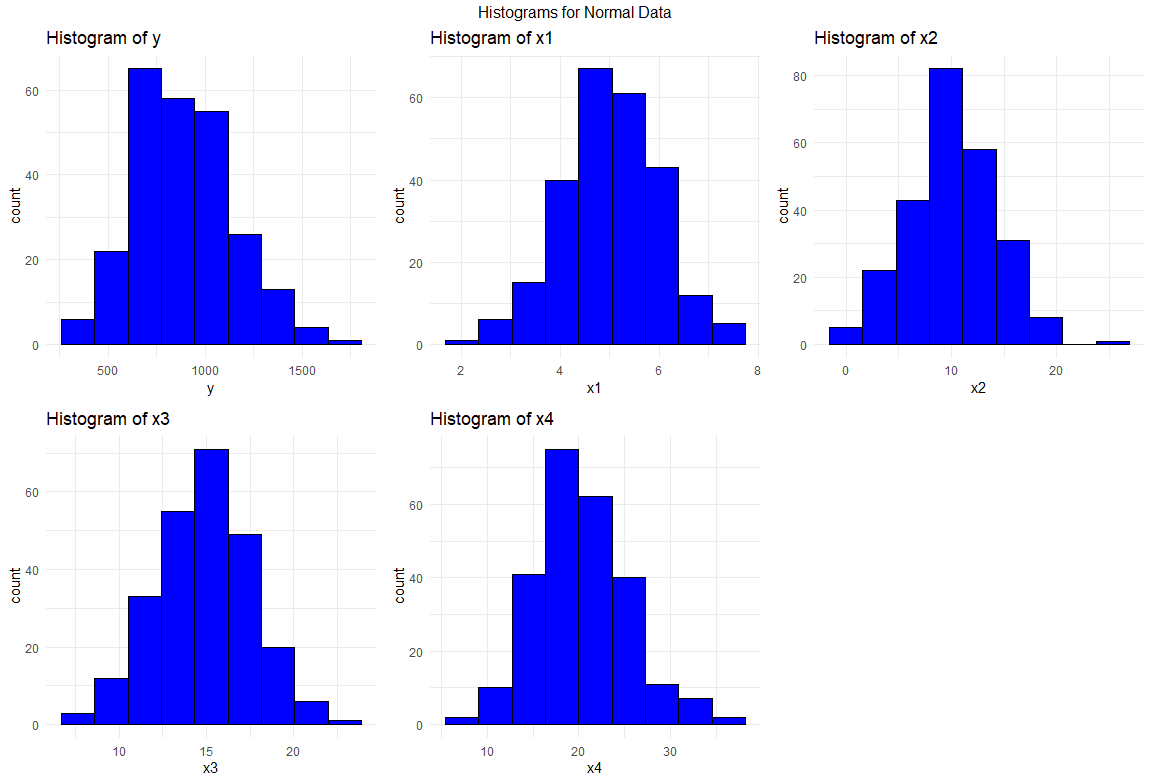
\includegraphics[width=14cm]{p2/7.png}
	\caption{his.homo}
	\label{fig:j06}
\end{figure}

\begin{figure}[h] 
	\centering
	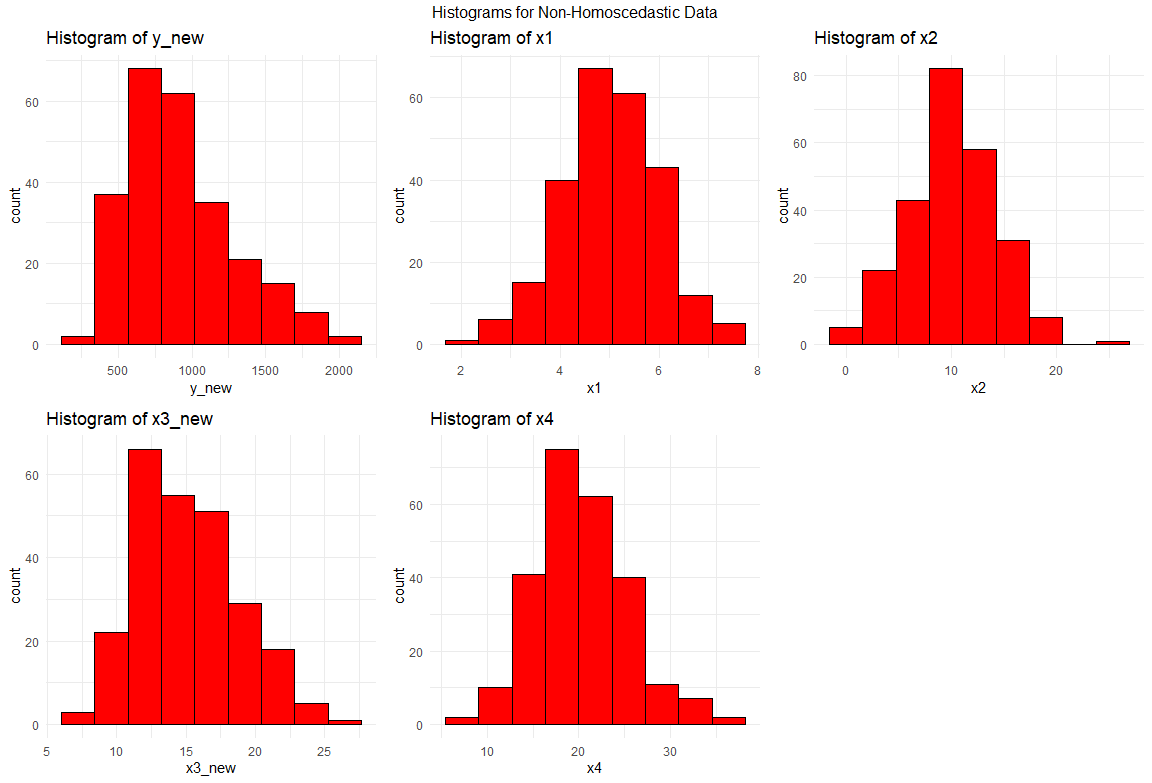
\includegraphics[width=14cm]{p2/8.png}
	\caption{his.hetro.}
	\label{fig:j06}
\end{figure}

	\newpage
	
	\section{Comparison between regressions}
	\newpage
	
	\section{Discussion}
	\newpage
	
	\section{Conclusion}
	\newpage
	
 	\section{Litteratur}
  
\end{document}
